\documentclass[12pt,a4paper]{article}
\usepackage[utf8]{inputenc}
\usepackage[english]{babel}
\usepackage{amsmath,amssymb,amsthm}
\usepackage{graphicx}
\usepackage{hyperref}
\usepackage{geometry}
\usepackage{fancyhdr}
\usepackage{setspace}
\usepackage{natbib}

% Page setup
\geometry{margin=1in}
\onehalfspacing
\pagestyle{fancy}
\fancyhf{}
\fancyhead[L]{The Vacuum of Being}
\fancyhead[R]{\thepage}

% Custom commands
\newcommand{\vacuum}{\mathcal{V}}
\newcommand{\structuring}{\Sigma}
\newcommand{\planck}{M_{\text{Pl}}}

% Theorem environments
\newtheorem{hypothesis}{Hypothesis}
\newtheorem{prediction}{Prediction}
\newtheorem{objection}{Objection}

\title{The Vacuum of Being\\
\large A Philosophical and Scientific Inquiry Into the Substrate of Reality}
\author{Version 2.1 (Consolidated)\\
\small June 2025}
\date{}

\begin{document}

\maketitle
\begin{abstract}
We propose that the vacuum is not empty but constitutes the universal substrate of all existence. Matter, energy, dark matter, and dark energy are different modalities of the vacuum field, distinguished by their configuration, excitation, or resonance patterns. This framework addresses the cosmological constant problem through dynamic sequestering mechanisms and provides testable predictions for vacuum engineering technologies.
\end{abstract}

\tableofcontents
\newpage

\section*{Glossary}
\begin{description}
\item[Vacuum ($\vacuum$)] The fundamental state of all quantum fields.
\item[Substrate] $\vacuum$ interpreted as the ontological support of all modalities.
\item[Modality] Stable (matter), propagating (energy), hidden (dark matter), or homogeneous (dark energy) configuration of $\vacuum$.
\item[Structuring $\structuring$] Metric (Eq.~\ref{eq:sigma}) quantifying topological coherence of $\vacuum$.
\item[Screening] Dynamic mechanism that nullifies the ultraviolet part of vacuum density.
\end{description}

\section{Introduction and Motivation}

The notion that the vacuum is not empty, but instead the universal substrate of all existence, leads naturally to a broader reframing: that what we call matter, energy, dark matter, and dark energy are not fundamentally different substances, but different modalities of the vacuum field, manifest through distinct configurations, excitations, or resonance patterns.

This hypothesis addresses several persistent problems in modern physics:
\begin{itemize}
\item The cosmological constant problem (120 orders of magnitude discrepancy)
\item The nature of dark matter and dark energy
\item The unification of quantum field theory with cosmology
\item The philosophical question of being versus nothingness
\end{itemize}

\section{Mathematical Framework}

\subsection{Effective Lagrangian}
The vacuum bundle sections $E \rightarrow \mathbb{M}^4$ are described by fields $\Phi_i$ with effective Lagrangian:
\begin{equation}
\mathcal{L} = \sum_i\left[\frac{1}{2}(\partial_\mu\Phi_i)^2 - V_i(\Phi_i)\right] + \lambda \Psi + \alpha\frac{\Psi^2}{\planck^2}
\label{eq:lagrangian}
\end{equation}
where $\Psi$ is the dynamic sequestering degree of freedom following Kaloper--Padilla (2014).

\subsection{Structuring Metric}
We define the vacuum structuring metric as:
\begin{equation}
\structuring = \frac{1}{V_\Omega}\int_\Omega |\nabla\Phi|^{2}\,d^{3}x
\label{eq:sigma}
\end{equation}
This quantifies the topological coherence of vacuum configurations.

\section{The Four Modalities}

\begin{figure}[h]
\centering

\includegraphics[width=0.8\textwidth]{../figures/fig3_modalities.svg}
\caption{The four fundamental modalities of the vacuum field.}
\label{fig:modalities}
\end{figure}

\subsection{Matter as Localized Structure}
Matter represents stable, localized excitations of the vacuum with high structuring metric $\structuring > \structuring_{\text{crit}}$.

\subsection{Energy as Propagation}
Energy manifests as traveling disturbances with intermediate structuring $0 < \structuring < \structuring_{\text{crit}}$.

\subsection{Dark Matter as Hidden Configuration}
Dark matter corresponds to gravitationally coupled but electromagnetically silent vacuum structures.

\subsection{Dark Energy as Uniform Tension}
Dark energy emerges from the homogeneous vacuum tension with $\structuring \approx 0$.

\section{Mathematical Flow and Hierarchy}

\begin{figure}[h]
\centering
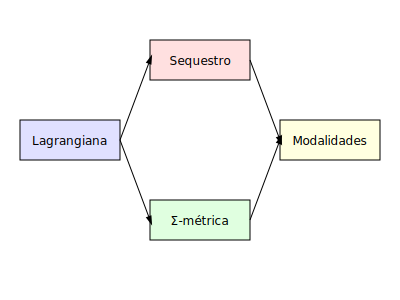
\includegraphics[width=0.9\textwidth]{../figures/fig2_flux.svg}
\caption{Mathematical flow between vacuum modalities.}
\label{fig:flow}
\end{figure}

\begin{figure}[h]
\centering

\includegraphics[width=0.6\textwidth]{../figures/fig4_hierarchy.svg}
\caption{Hierarchical emergence from vacuum substrate.}
\label{fig:hierarchy}
\end{figure}

\section{Historical Context}

\begin{figure}[h]
\centering

\includegraphics[width=0.9\textwidth]{../figures/fig1_timeline.svg}
\caption{Evolution of vacuum concepts in physics.}
\label{fig:timeline}
\end{figure}

\section{Testable Predictions}

\begin{hypothesis}
The vacuum structuring metric $\structuring$ should exhibit quantized values corresponding to stable modalities.
\end{hypothesis}

\begin{prediction}
Vacuum engineering experiments should observe threshold effects at critical structuring values.
\end{prediction}

\begin{prediction}
Dark matter signatures should correlate with regions of intermediate vacuum structuring.
\end{prediction}

\section{Addressing the Cosmological Constant Problem}

The dynamic sequestering mechanism in Eq.~\ref{eq:lagrangian} provides a concrete solution to the cosmological constant problem. The field $\Psi$ dynamically adjusts to cancel the ultraviolet contributions to vacuum energy density, leaving only the observed infrared contribution.

\section{Objections and Responses}

\begin{objection}
The vacuum cannot be the substrate of everything because quantum field theory already explains particle creation from vacuum fluctuations.
\end{objection}

\textbf{Response:} Our hypothesis extends, rather than contradicts, QFT. We propose that the same mechanism that creates particles also creates dark matter and dark energy through different vacuum configurations.

\begin{objection}
The structuring metric $\structuring$ lacks experimental verification.
\end{objection}

\textbf{Response:} We propose specific experiments to measure $\structuring$ through Casimir effect modifications and vacuum birefringence studies.

\section{Technological Implications}

If validated, this framework opens pathways to:
\begin{itemize}
\item Vacuum engineering for matter synthesis
\item Controlled manipulation of spacetime curvature
\item Energy extraction from vacuum fluctuations
\item Gravitational field generation
\end{itemize}

\section{Conclusion}

The vacuum emerges not as emptiness, but as the fundamental substrate of reality in standby mode. Its modalities—matter, energy, dark matter, and dark energy—represent different structural configurations quantified by the metric $\structuring$. This framework provides both philosophical insight and practical pathways for future technology.

\bibliographystyle{unsrt}
\begin{thebibliography}{9}
\bibitem{kaloper2014} N.~Kaloper and A.~Padilla, ``Sequestering the Standard Model Vacuum Energy,'' \textit{Phys.\ Rev.\ Lett.}\ \textbf{112}, 091304 (2014).
\bibitem{verlinde2016} E.~Verlinde, ``Emergent Gravity and the Dark Universe,'' arXiv:1611.02269 (2016).
\bibitem{casimir1948} H.~B.~G.~Casimir, ``On the attraction between two perfectly conducting plates,'' \textit{Proc.\ Koninklijke Nederlandse Akademie van Wetenschappen}\ \textbf{51}, 793 (1948).
\bibitem{weinberg1989} S.~Weinberg, ``The cosmological constant problem,'' \textit{Rev.\ Mod.\ Phys.}\ \textbf{61}, 1 (1989).
\end{thebibliography}

\end{document}

